\documentclass[tikz]{standalone}
\usepackage{tikz}
\usepackage{amsmath}
\usepackage{amsfonts}
\usepackage{amssymb}
\usetikzlibrary{arrows.meta, calc}

\colorlet{l1color}{blue!50!cyan}
\colorlet{l2color}{red!60!orange}

\begin{document}
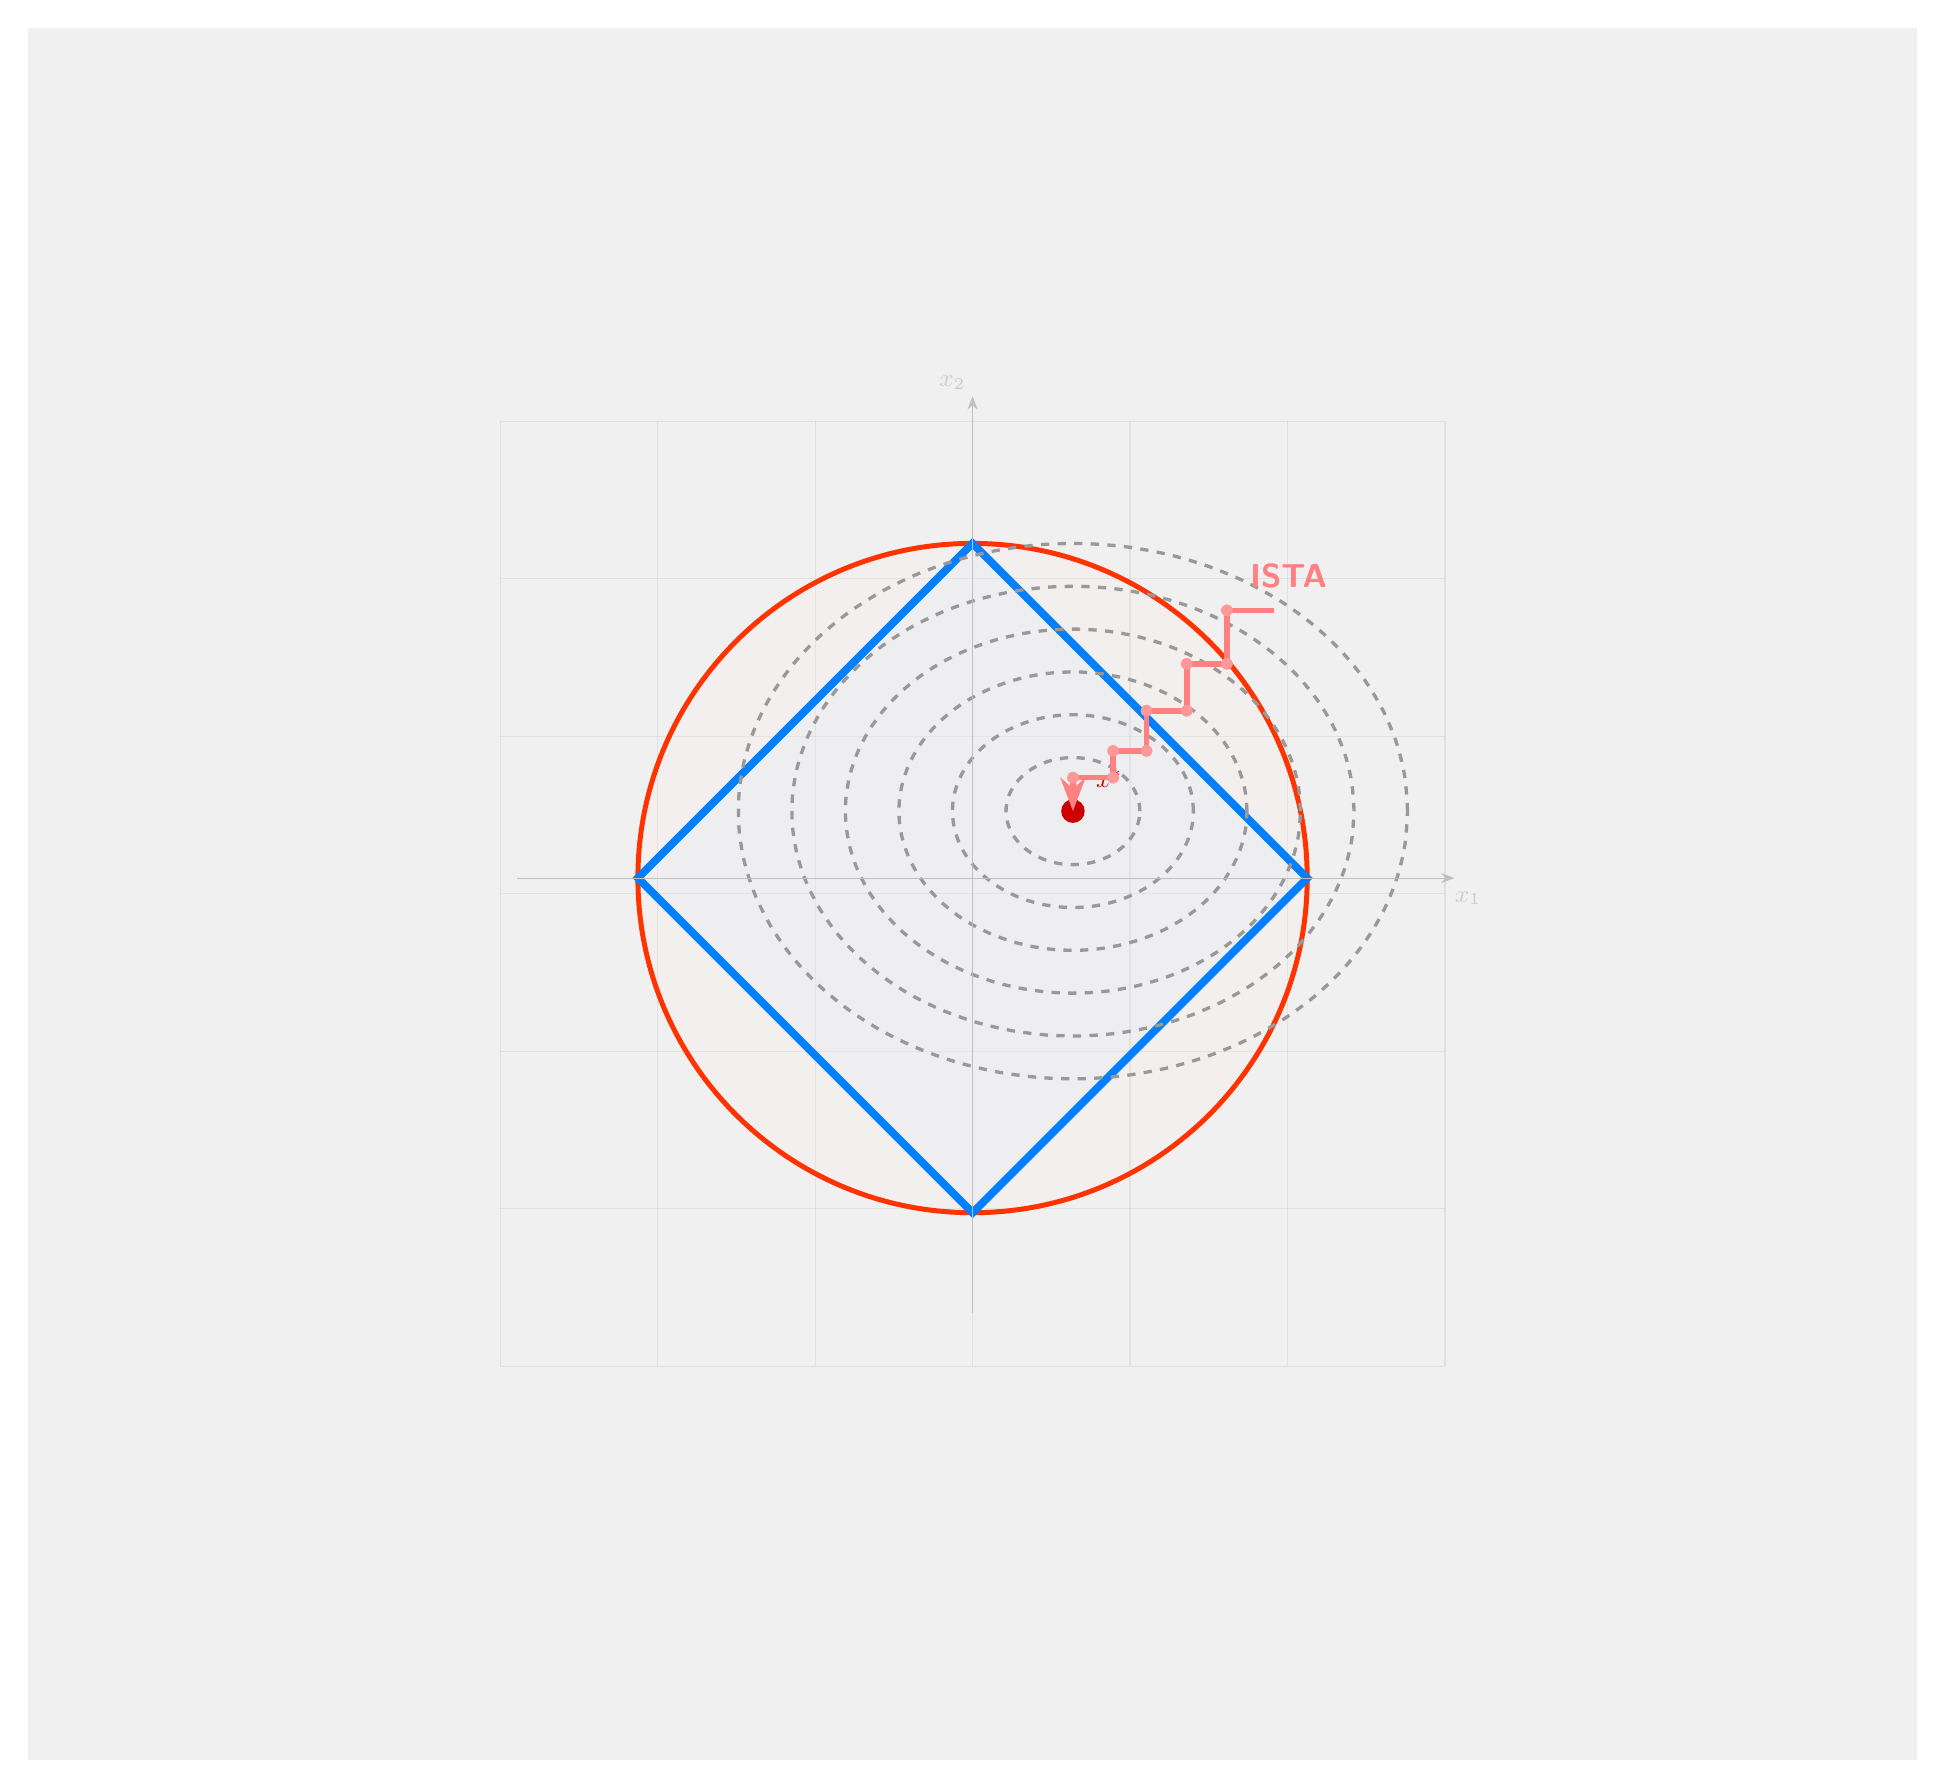
\begin{tikzpicture}[>=Stealth, scale=1.0]

  \fill[gray!12] (-12,-11) rectangle (12,11);

  \begin{scope}[opacity=0.06]
    \foreach \x in {-6,-4,-2,0,2,4,6} {
      \draw[black, thin] (\x,-6) -- (\x,6);
      \draw[black, thin] (-6,\x) -- (6,\x);
    }
  \end{scope}

  \begin{scope}[shift={(0,0.2)}, scale=0.85]

    \fill[l2color!10, opacity=0.15] (0,0) circle (5.0);
    \draw[l2color, line width=1.8pt] (0,0) circle (5.0);

    \fill[l1color!15, opacity=0.15]
      (5.0,0) -- (0,5.0) -- (-5.0,0) -- (0,-5.0) -- cycle;
    \draw[l1color, line width=2.8pt]
      (5.0,0) -- (0,5.0) -- (-5.0,0) -- (0,-5.0) -- cycle;

    \foreach \r in {1.0, 1.8, 2.6, 3.4, 4.2, 5.0} {
      \draw[black!40, line width=1.2pt, dashed, smooth]
        plot[domain=0:360, samples=50, variable=\t]
        ({1.5 + 1.0*\r*cos(\t)}, {1.0 + 0.8*\r*sin(\t)});
    }

    \fill[red!80!black] (1.5, 1.0) circle (5pt);
    \node[red!80!black, font=\small, anchor=south west] at (1.7, 1.2) {$x^*$};

    \draw[red!50, line width=2.0pt, ->]
      (4.5, 4.0) -- (3.8, 4.0) -- (3.8, 3.2) -- (3.2, 3.2)
      -- (3.2, 2.5) -- (2.6, 2.5) -- (2.6, 1.9) -- (2.1, 1.9)
      -- (2.1, 1.5) -- (1.5, 1.5) -- (1.5, 1.0);

    \node[red!50, font=\large\bfseries\sffamily, anchor=south west]
      at (4.0, 4.2) {ISTA};

    \foreach \pt in {(3.8,4.0), (3.8,3.2), (3.2,3.2), (3.2,2.5), (2.6,2.5), (2.6,1.9), (2.1,1.9), (2.1,1.5), (1.5,1.5)} {
      \fill[red!40] \pt circle (2.5pt);
    }

    \draw[->, black!25, thin] (-6.8,0) -- (7.2,0);
    \draw[->, black!25, thin] (0,-6.5) -- (0,7.2);
    \node[black!20, font=\small] at (7.4,-0.3) {$x_1$};
    \node[black!20, font=\small] at (-0.3,7.4) {$x_2$};

  \end{scope}

\end{tikzpicture}
\end{document}